\newpage
\section{Задание 5} 
{\bf\large Условие} \\
Провести полное исследование функций и построить их графики.
\begin{enumerate}
    \item 
    \begin{equation*}
        \begin{cases}
            x = \frac{3t^2 +1}{3t} \\
            y = t + \frac{t^2}{3}
        \end{cases}
    \end{equation*}
    \item 
    \[
        y = \arccos{\frac{2x}{1+x^2}} - \frac{2x}{5}
    \]
    \item 
    \[
        y = (1-x)e^{3x+1}
    \]
\end{enumerate}
{\bf\large Ход решения} \\
\begin{enumerate}
    \item 
    \begin{equation*}
        \begin{cases}
            x = \frac{3t^2 +1}{3t} \\
            y = t + \frac{t^2}{3}
        \end{cases}
    \end{equation*}
    Найдем область определения функции $D(f)$: \\
    $y(t)$ - существует всегда, рассмотрим чему не может равняться $x(t)$:\\
    $x(t) = \frac{3t^2 +1}{3t} = t + \frac{1}{3t}$ - не достигает каких-то значений около нуля, найдем их через локальный минимум/максимум: \\
    $x'(t) = 1 - \frac{1}{3t^2}$ - не существует в нуле как и сама функция $x(t)$,
    $x'(t) = 0 \Rightarrow 1 - \frac{1}{3t^2} = 0 \Rightarrow t = \pm \sqrt{\frac{1}{3}}$ \\
    Подставив различные значения, получим, что: $\frac{1}{\sqrt{3}}$ - лок. минимум, $-\frac{1}{\sqrt{3}}$ - лок. максимум \\
    $x(\frac{1}{\sqrt{3}}) = \frac{2}{\sqrt{3}}$, $x(-\frac{1}{\sqrt{3}}) = -\frac{2}{\sqrt{3}}$ \\
    То есть $D(f) = (-\infty,-\frac{2}{\sqrt(3)}] \cup [\frac{2}{\sqrt(3)},+\infty)$ \\
    Найдем сначала асимптоты кривой. Будем искать наклонные асимптоты в виде $y = kx + b$. Переменная $x$ стремится к бесконечности, когда $t\rightarrow 0$ или $t\rightarrow \pm \infty$. 
    При $t \rightarrow \pm \infty$ переменная $y$ тоже будет стремится к бесконечности, при этом: \\
    \[
        \lim_{t\rightarrow \infty }{\frac{y(t)}{x(t)}} = \lim_{t\rightarrow \infty }{\frac{3t(3t+t^2)}{3(3t^2+1)}}=\lim_{t\rightarrow \infty }{\frac{3t^2+t^3}{3t^2+1}} = \infty
    \] 
    И к тому же $x\rightarrow\infty$, значит, при стремленни $t\rightarrow\infty$ нет ни наклонной, не вертикальной асимптоты. \\
    Расмотим случай $t\rightarrow \pm 0$: \\
    \[
        \lim_{t\rightarrow0+}{\frac{y(t)}{x(t)}}=\lim_{t\rightarrow0+}{\frac{3t^2+t^3}{3t^2+1}}=\frac{0+0}{0+1}=0
    \]
    \[
        \lim_{t\rightarrow0-}{\frac{y(t)}{x(t)}}=\lim_{t\rightarrow0-}{\frac{3t^2+t^3}{3t^2+1}}=0
    \]
    При этом:
    \[
        \lim_{t\rightarrow0}{y(t)} = \lim_{t\rightarrow0}{t+\frac{t^2}{3}} = 0
    \]
    То есть при $t\rightarrow 0$ есть горизонтальная асимптота $y = 0$\\
    Исследуем производные функций $y(t)$ и $x(t)$, для того, чтобы понять, как ведет себя функция: \\
    \begin{center}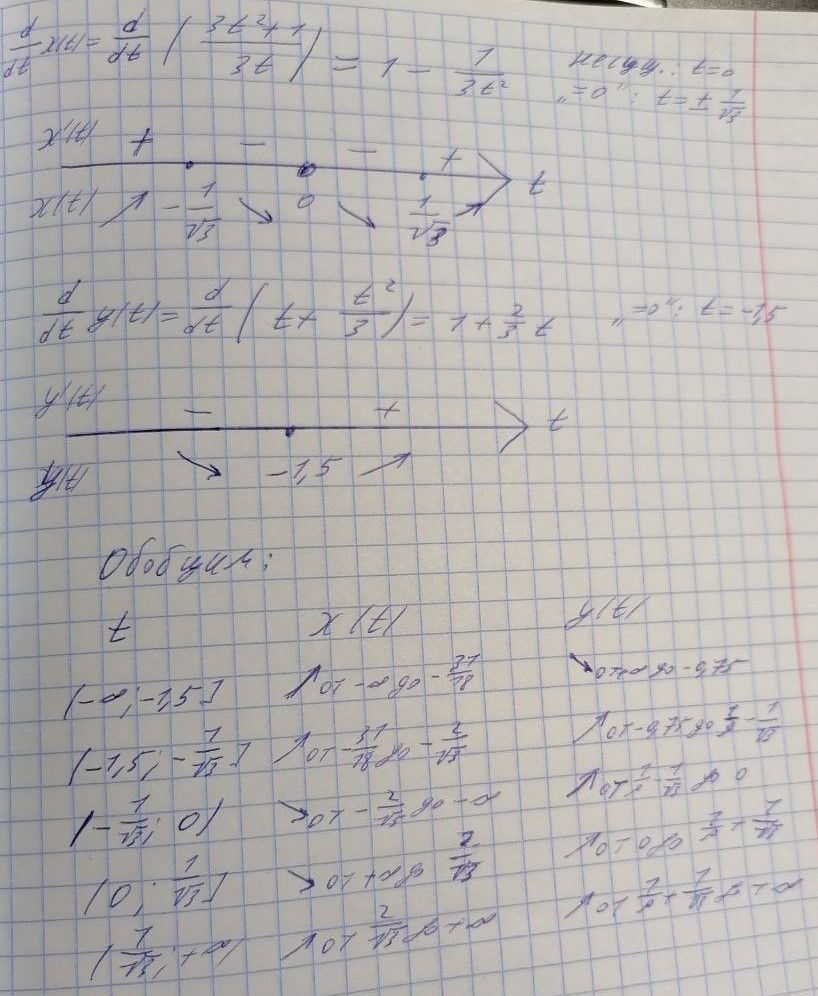
\includegraphics[width=0.7\linewidth]{13.jpg}\end{center}
    \begin{center}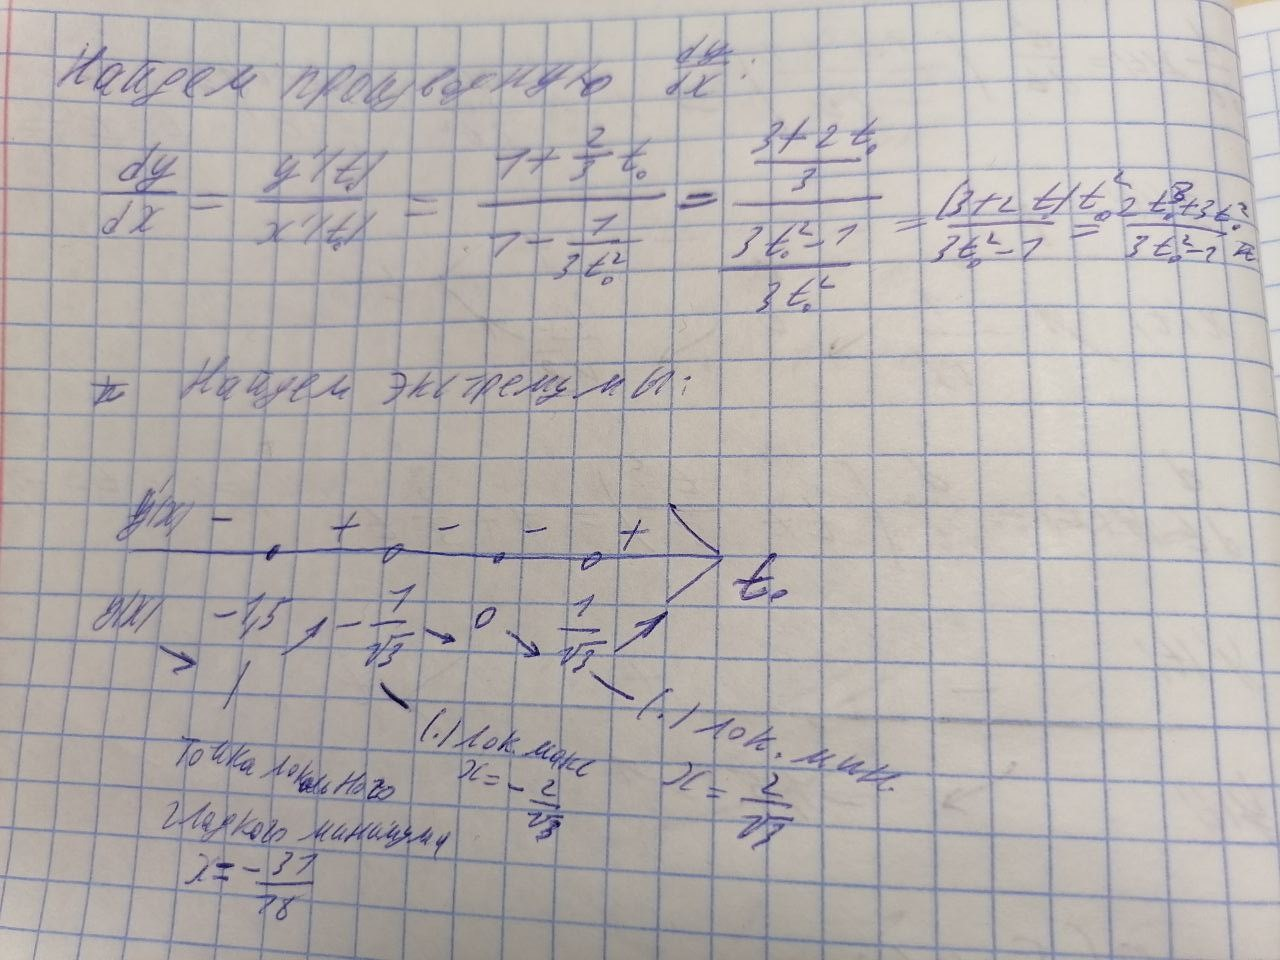
\includegraphics[width=0.7\linewidth]{14.jpg}\end{center}
    \begin{center}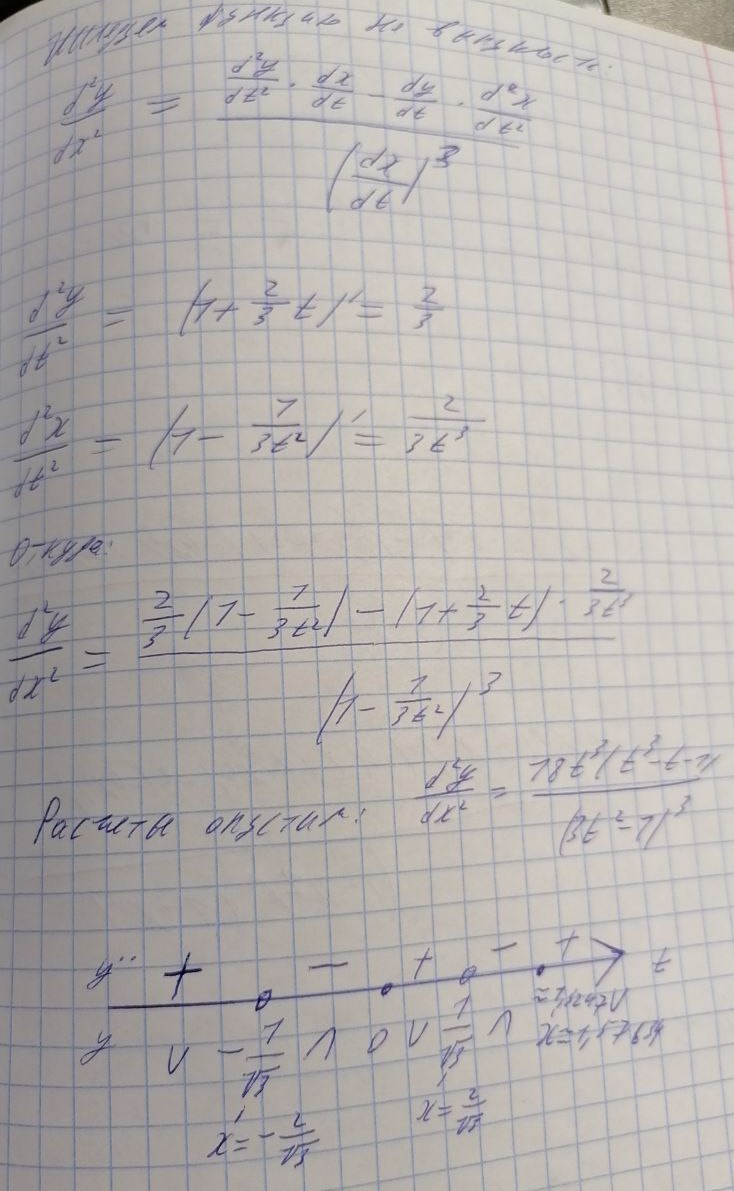
\includegraphics[width=0.7\linewidth]{15.jpg}\end{center}
    После проведенных вычислений становится понятно, что функция не является четной/нечетной или периодической. 
    Построим её график:
    \begin{center}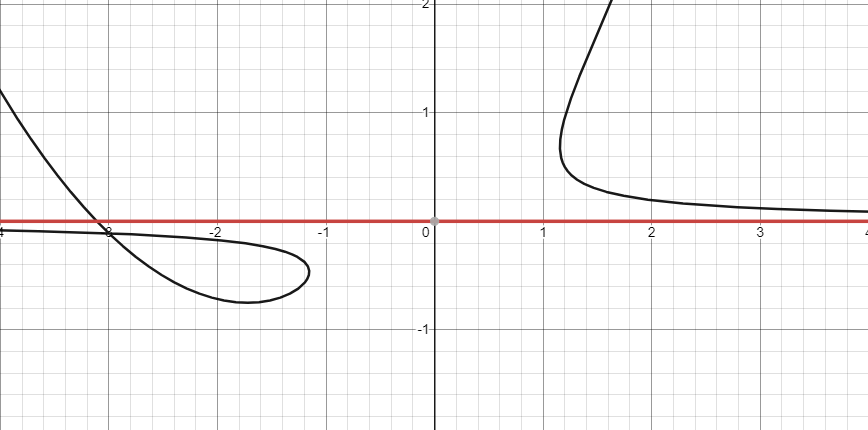
\includegraphics[width=0.7\linewidth]{16.png}\end{center}
    \item 
    \[
        y = \arccos{\frac{2x}{1+x^2}} - \frac{2x}{5}
    \]
    Найдем область определения функции $D(f)$: \\
    \begin{equation*}
        \left|\frac{2x}{1+x^2}\right| \leq 1 
        \Rightarrow |2x| \leq 1+x^2 
        \Rightarrow \begin{cases}
            2x \leq 1+x^2 \\
            2x \geq -1 - x^2 
        \end{cases} \Rightarrow
        \begin{cases}
            0 \leq (1-x)^2 \\
            0 \geq -(1 + x)^2 
        \end{cases}
    \end{equation*}
    Что выполняется всега, $D(f) = \mathbb{R}$ \\
    Функция не является ни четной, ни нечетной, а также не является периодичной. \\
    Исследуем ее на монотонность и экстремумы. Для этого найдем производную: \\
    $y'=-\frac{1}{\sqrt{1-\left(\frac{2x}{1+x^2}\right)^2}}\cdot\frac{2(1+x^2)-2x(2x)}{(1+x^2)^2}-\frac{2}{5} = \frac{1}{\sqrt{1-\left(\frac{2x}{1+x^2}\right)^2}}\cdot\frac{2x^2 -2}{(1+x^2)^2}-\frac{2}{5}= \frac{(1+x^2)}{\sqrt{(1+x^2)^2-4x^2}}\cdot\frac{2x^2 -2}{(1+x^2)^2}-\frac{2}{5}=\frac{1}{|x-1||x+1|}\cdot\frac{2x^2 -2}{1+x^2}-\frac{2}{5}$ \\
    Найдем точки "подозреваемые" на экстремум: \\
    Случай 1 ($y'$ - не существует): 
    $|x-1||x+1|=0$\\
    Откуда $x = 1$ или $x = -1$\\
    Случай 2 ($y'=0$):\\
    \begin{gather*}
    \frac{1}{|x-1||x+1|}\cdot\frac{2x^2 -2}{1+x^2}-\frac{2}{5}=0 \\
    \frac{x^2 -1}{1+x^2}=\frac{|x-1||x+1|}{5} \\
    5x^2 -5=|x^4-1| \\
    \begin{cases}
        |x| \geq 1 \\
        \left[
        \begin{gathered} 
            5x^2 -5 = x^4 -1 \\
            \hspace{7pt} 5x^2 -5 = -x^4 +1 \\
        \end{gathered} 
        \right.
    \end{cases} \\
    \begin{cases}
        |x| \geq 1 \\
        \left[
        \begin{gathered} 
            x^2=1 \\
            x^2=4\\
            x^2=1\\
            \hspace{7pt} x^2=-6
        \end{gathered} 
        \right.
    \end{cases} 
    \end{gather*}
    Итого $x=\pm 1,\pm 2$ \\
    По \sout{desmos} методу интерваллов отпределим, что -1 и 2 - точки лок. максимума, 1 и -2 - точки лок. минимума \\
    %Вычислим экстремальные значения функции: $y(-1) = \pi + \frac{2}{5}, y(1) = -\frac{2}{5},$\\$ y(-2) = \arccos{-\frac{4}{5}}+\frac{4}{5},y(2) = \arccos{\frac{4}{5}}-\frac{4}{5}$
    Найдем асимптоты функции: \\
    При $x\rightarrow \infty$, $y$ тоже $\rightarrow \infty$, других асимптот нет, так как $\arccos{\frac{2x}{1+x^2}}$ - что-то ограниченное, а $-\frac{2x}{5}\rightarrow \infty$ только при $x\rightarrow \infty$\\
    Найдем наклонную асимптоту $y=kx+b$ для $\pm \infty$:\\
    \[\lim_{x\rightarrow +\infty}{\frac{\arccos{\frac{2x}{1+x^2}} - \frac{2x}{5}}{x}}=
    0+\left(-\frac{2}{5}\right)=-\frac{2}{5}
    \]
    \[\lim_{x\rightarrow -\infty}{\frac{\arccos{\frac{2x}{1+x^2}} - \frac{2x}{5}}{x}}=
    0+\left(-\frac{2}{5}\right)=-\frac{2}{5}
    \]
    При этом найдем $b$:
    \[\lim_{x\rightarrow +\infty}{\left(\arccos{\frac{2x}{1+x^2}} - \frac{2x}{5} - \left(-\frac{2x}{5}\right)\right)} = 
    \lim_{x\rightarrow +\infty}{\arccos{\frac{2x}{1+x^2}}} = \arccos{0} = \frac{\pi}{2}
    \]
    \[\lim_{x\rightarrow -\infty}{\left(\arccos{\frac{2x}{1+x^2}} - \frac{2x}{5} - \left(-\frac{2x}{5}\right)\right)} = 
    \lim_{x\rightarrow -\infty}{\arccos{\frac{2x}{1+x^2}}} = \arccos{0} = \frac{\pi}{2}
    \]
    То есть полученная асимптота: $y = -\frac{2}{5}x+\frac{\pi}{2}$
    Исследуем функцию на выпуклость/вогнутость: \\
    \begin{center}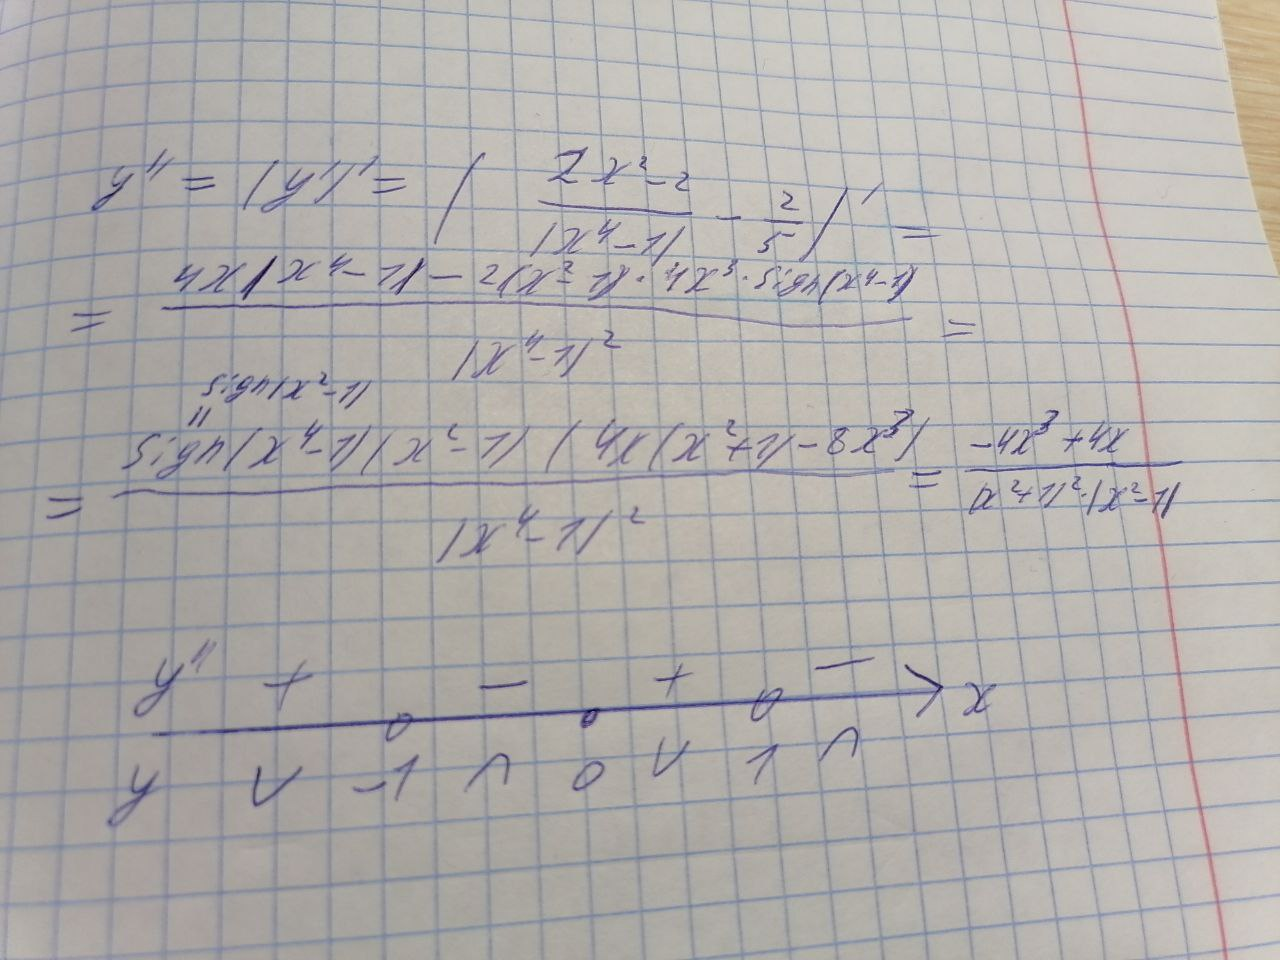
\includegraphics[width=0.7\linewidth]{17.jpg}\end{center}
    Построим график: \\
    \begin{center}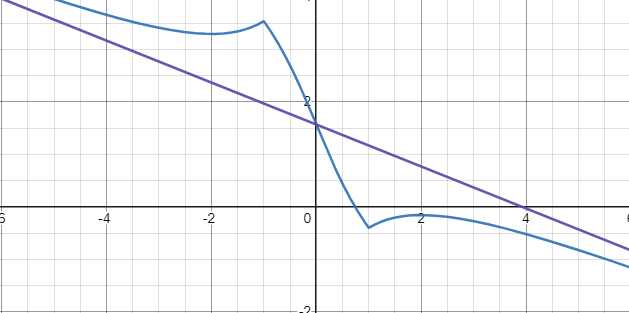
\includegraphics[width=0.7\linewidth]{18.png}\end{center}
    \item 
    \[
        y = (1-x)e^{3x+1}
    \]
    Область определения функции: $\mathbb{R}$ \\
    Функция не является ни четной, ни нечетной, а также не является периодичной. \\
    Исследуем ее на монотонность и экстремумы. Для этого найдем производную: \\
    \begin{center}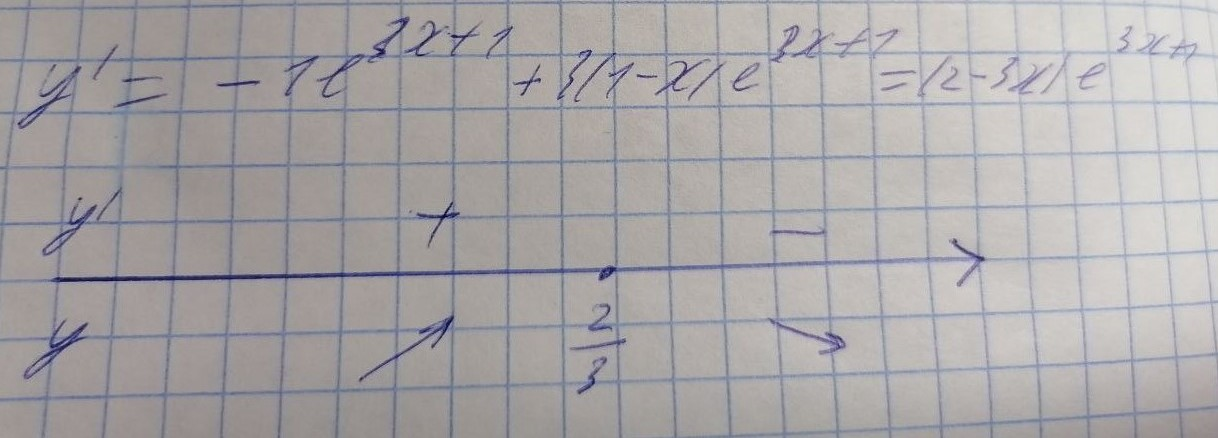
\includegraphics[width=0.7\linewidth]{19.jpg}\end{center}
    После, найдем асимптоты к графику:\\
    \begin{center}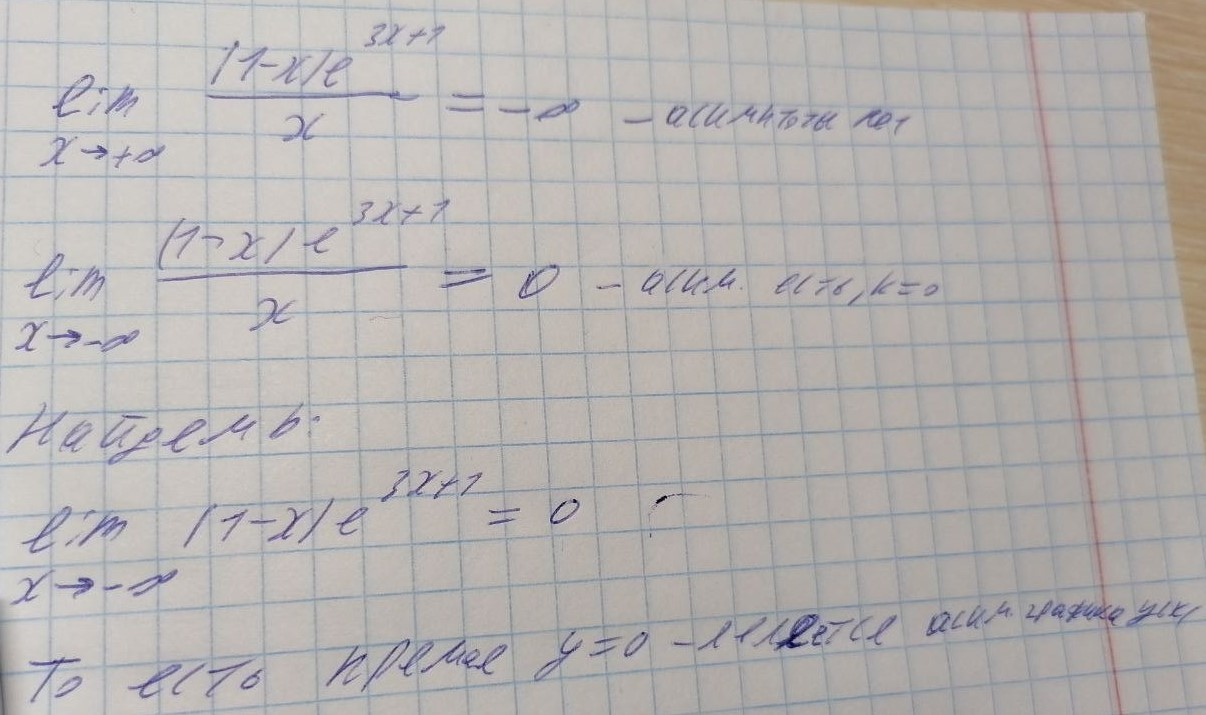
\includegraphics[width=0.7\linewidth]{20.jpg}\end{center}
    А следом, исследуем на выпуклость/вогнутость:\\
    \begin{center}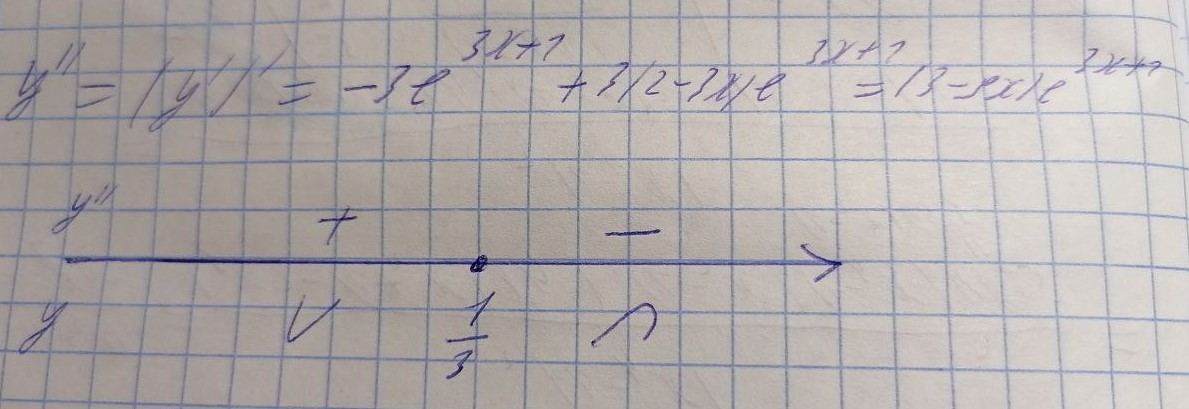
\includegraphics[width=0.7\linewidth]{21.jpg}\end{center}
    Построим график:\\
    \begin{center}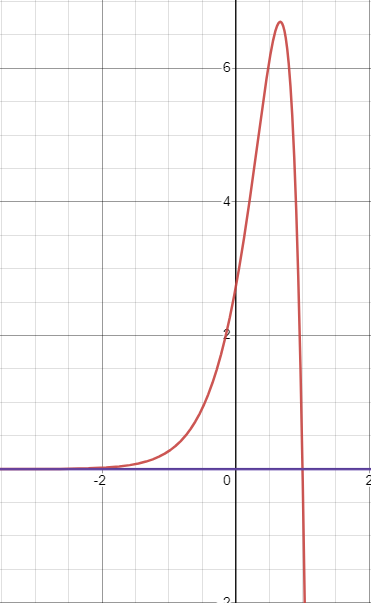
\includegraphics[width=0.7\linewidth]{22.png}\end{center}
\end{enumerate}